\chapter{Physics Objects}
\label{sec:reco}
\section{Introduction}
In the previous chapter details of the \ac{CMS} detector were presented. We
shall now begin to discuss the algorithms used to reconstruct analysis level
objects and quantities which will be of fundamental importance in later
chapters. The objects of primary interest for these purposes are leptons, jets
and missing energy. The offline reconstruction algorithms used to reconstruct
each object will be presented, along with issues and properties related to data
analysis. Some details of the reconstruction performance at \ac{CMS} will also
be shown. Finally, the \acf{PF} algorithm, which provides a global
reconstruction of the event, will be explained in some detail. As will be seen,
\ac{PF} combines tracking and calorimeter measurements to provide excellent
reconstruction of jets and missing energy.

\section{Leptons}
The reconstruction of electrons and muons at \ac{CMS} will now be
described. Since tau leptons are not used by either of the analyses presented in
this work, their reconstruction will not be described here. The interested
reader is directed to relevant literature~\cite{cms_pf_tau_id,tau_reco_cms}.

\subsection{Muons}
\label{sec:reco_muons}
The full details of muon reconstruction at CMS are presented
in~\cite{cms_mu_reco,cms_mu_pas,mu_align_pas}. A brief overview will be presented here,
focusing on the aspects pertinent to the following analysis chapters. Muons are
reconstructed in both the muon chambers and the silicon tracker. To exploit this
redundancy in the measurement, several reconstruction algorithms have been
developed.

\subsubsection{Tracker Muons}
\emph{Tracker muons} begin as tracks in the silicon tracker. All tracks with a
$\Pt > \unit{0.5}{\GeV}$ and $p > \unit{2.5}{\GeV}$ are considered as muon
candidates and extrapolated to the muon stations, accounting for expected energy
loss and multiple scattering effects. If at least one muon track segment matches
the extrapolated tracker track, a tracker muon is reconstructed. This algorithm
is more efficient at low momentum ($p < \unit{5}{\GeV}$) since it requires only
a single segment in the muon chambers.

\subsubsection{Standalone Muons}
\emph{Standalone muons} are based solely on measurements in the muon
chambers. The hits in each chamber are fit individually to obtain seeds -- a
position and direction vector along with an estimate of the transverse
momentum. These form the basis of a track fit in the muon chambers based on the
Kalman-filter technique~\cite{kalman_filter}. The fit is constrained to the
vertex in order to reject cosmic ray muons. Since much of the calibration and
validation work for the muon system was performed using cosmic rays, a separate
algorithm was developed for this purpose~\cite{cms_mu_reco_cosmic}.

\subsubsection{Global Muons}
\emph{Global muons} are an extension of standalone muons to include measurements
in the silicon tracker. For muons with a transverse momentum below $\approx$
\unit{200}{\GeV}, the tracker provides a better momentum resolution. For higher
momentum muons, the tracks become straighter and the momentum measurement
increasingly affected by uncertainty in the position measurement. In this
regime, inclusion of hits in the muon chambers effectively benefits from the
large lever arm and \unit{3.8}{\tesla} magnetic field in the region between the
silicon tracker and the muon chambers.

For each standalone muon, the set of tracker tracks is searched and the best
matching candidate selected. For each pairing found in this way, a Kalman-filter
fit is again performed, this time using hits from both the silicon tracker and
the muon chambers. This fit accounts for average expected energy losses,
magnetic field and multiple scattering effects. The tracks reconstructed by this
procedure become global muons. Once again, certain modifications are required for
reconstructing cosmic ray muons -- for instance in the case that cosmic muons
traverse the entire detector, leaving two standalone muons on either side of
\ac{CMS}.

\subsubsection{Merging}
Reconstructed muons from each of the algorithms detailed above are then merged
into a single list of muon candidates. Candidates reconstructed as both global
and tracker muons are merged. Standalone muon tracks are merged with tracker
muons if they share a muon segment. The fit results from each algorithm are
retained.

An analysis is then able to tune its identification cuts to meet certain
efficiency or purity requirements for a particular kinematic range. A number of
predefined selections are available.
\begin{itemize}
\item ``Soft muons'' are required to be reconstructed as tracker muons with a muon
  segment in the outermost station matching the position and direction expected
  from extrapolation of the track.
\item ``Global muons'' are simply those muons reconstructed by the global muon
  algorithm described above.
\item ``Tight muons'' must be reconstructed as both a global muon and a tracker muon
  with a series of additional requirements: a $\Pt > \unit{3}{\GeV}$, a global
  muon track fit with a normalised $\chisq < 10$, at least two muon stations
  with matching muon segments, at least 10 hits in the silicon tracker (with at
  least 1 pixel hit) and a transverse impact parameter $\dxy <
  \unit{2}{\milli\metre}$. This selection significantly suppresses
  decays-in-flight at the cost of a small loss in efficiency for prompt muons.
\end{itemize}

\fig~\ref{fig:reco_muon_perf} shows the muon transverse momentum resolution
as a function of muon \Pt. 

\begin{figure}[h!]
  \centering
  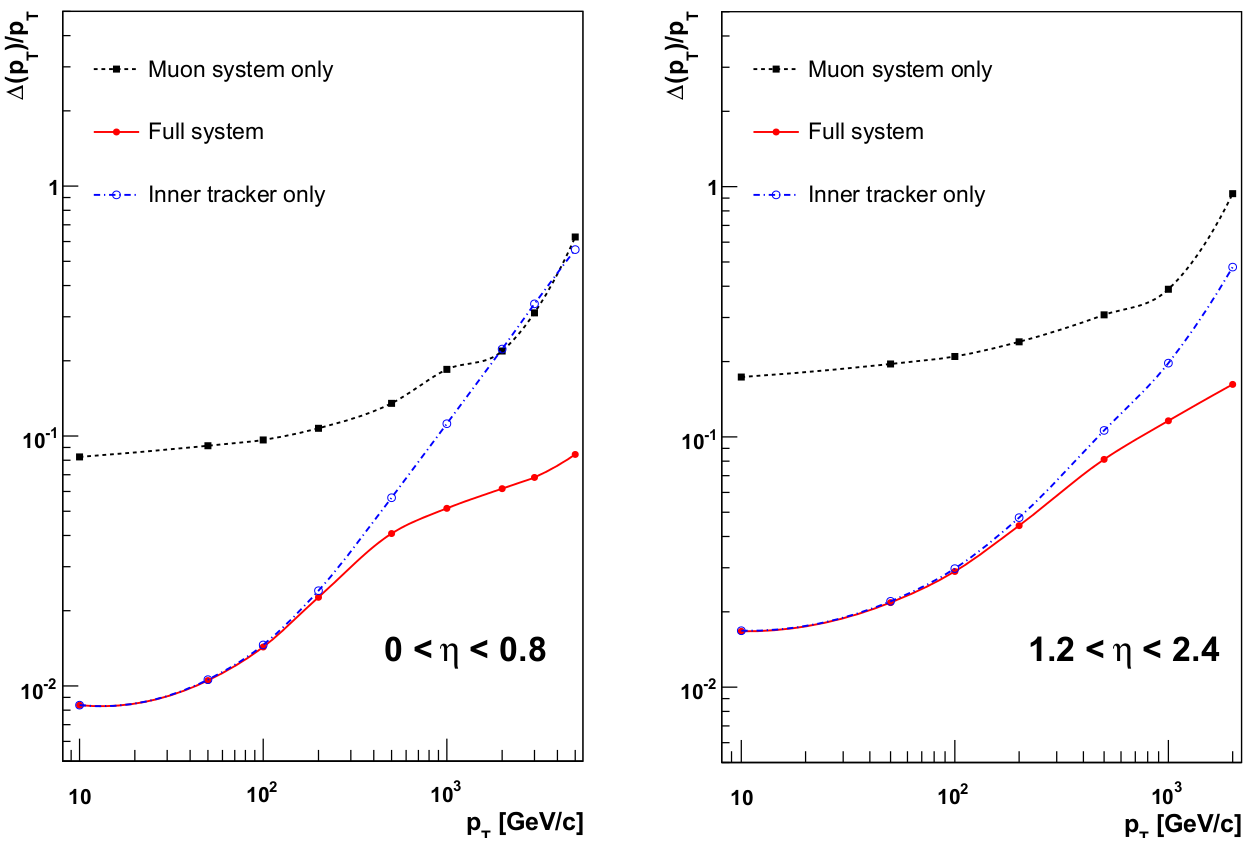
\includegraphics[width=0.8\textwidth]{fig/muon_perf}
  \caption[Muon transverse momentum resolution]{Muon transverse
    momentum resolution as a function of transverse momentum shown for
    the muon system only, the inner tracking only and both. The left
    figure is for $|\eta|<0.8$ and the right figure for
    $1.2<|\eta|<2.4$~\cite{cms_jinst}.}
  \label{fig:reco_muon_perf}
\end{figure}



\subsection{Electrons}
\label{sec:reco_electrons}
Electron reconstruction at \ac{CMS} makes use of measurements from both the
silicon tracker and the \ac{ECAL}. In the case of \ac{CMS}, the large amount of
material in the tracker causes electrons to radiate a large fraction of their
energy before reaching the \ac{ECAL} -- 50\% of electrons radiate more than 50\%
of their energy in this way. To obtain an accurate measurement of the electron
energy, this energy, radiated in the form of bremsstrahlung photons, must be
reconstructed correctly.

\subsubsection{Reconstruction}
Electron seeds are derived using two separate algorithms: \emph{tracker-driven}
and \emph{\ac{ECAL}-driven}~\cite{cms_ele_reco}. The tracker-driven algorithm was
developed for the purposes of the \ac{PF} algorithm. It is most suitable for
low-\Pt electrons and electrons produced inside jets. Seeds are found by
extrapolating \ac{GSF} tracks in the tracker from their outermost measurement to
the \ac{ECAL}. If a matching cluster is found, a tracker-driven seed is
created~\cite{cms_pf_pas3}.

\ac{ECAL}-driven seeds begin with the reconstruction of \ac{ECAL}
``superclusters'' with transverse energy, $\Et > \unit{4}{\GeV}$. A supercluster
is a group of one or more \ac{ECAL} clusters. It is formed to account for the
narrow $\eta$ width and spread in $\phi$ caused by the bending effect of the
\ac{CMS} magnet on electrons radiating in the
tracker~\cite{cms_ele_reco_pas}. These superclusters are then matched to track
seeds having two or three hits in the inner layers of the tracker. Electron
tracks are built from these track seeds. Trajectories are calculated accounting
for energy loss in the tracker. These are then fit with a \ac{GSF}~\cite{gsf}.

Candidates found only by the tracker-driven method must pass a pre-selection
based on a multivariate analysis~\cite{cms_pf_pas3}. Candidates found by the
\ac{ECAL}-driven algorithm are pre-selected by imposing an angular matching
requirement between the \ac{GSF} track and the supercluster. \ac{ECAL}-driven
seeds failing this matching requirement, but selected by the track-driven
multivariate pre-selection, are kept.

As described in \sec~\ref{sec:expt_laser_monitoring}, electron energies are
corrected to account for changes in the transparency of the \ac{ECAL}
crystals. For the \PW polarisation measurement, a set of ``ad-hoc'' corrections
were calculated from fits to the \PZ mass. For the \ac{SUSY} search analysis,
more sophisticated corrections were available~\cite{laser_monitoring}.

\subsubsection{Electron Identification}
\label{sec:reco_electron_id}
The large bremsstrahlung-induced energy loss, coupled with larger backgrounds
from jets and photons, means that electrons at \ac{CMS} are fundamentally less
well-defined objects than muons. There is therefore a much larger space to
trade-off between signal efficiency and purity. Whilst more complex selection
procedures are available (e.g. a multivariate approach), a simple cut-based
selection was chosen for the measurement of the \PW
cross-section~\cite{cms_pas_ewk_10_002,simple_eleid_web} and has been used in
this work. The variables have been chosen for their background rejection
capabilities but also for robustness during the early data-taking period.

A number of ``working points'' have been defined, each offering a fixed signal
efficiency, as measured in a simulated \Wenu sample. In each case, the cuts were
chosen to optimise background rejection power. These cuts were optimised
independently in the \ac{CMS} barrel and endcaps.

The cut variables used are described below, with cut-values for each working
point shown in Table~\ref{tbl:reco_electronid}.
\begin{itemize}
\item \sigmaieta is a measure of the \ac{RMS} shower width of the electron
  in the $\eta$ direction.
\item \deltaphiin and \deltaetain represent the angular separation between the
  trajectory of the \ac{GSF} track and the \ac{ECAL} supercluster.
\item Tracker, \ac{ECAL} and \ac{HCAL} isolation quantities summed in a cone
  $\Delta R < 0.3$~\cite{lepton_isolation_an}. The energy deposits and track
  associated with the lepton are removed. A threshold of \unit{700}{\MeV} is
  applied to the tracks contributing to the sum. Similarly, in the \ac{ECAL}, a
  zero-suppression cut is applied (\unit{0.08}{\GeV} in \ac{EB} and
  \unit{0.1}{\GeV} in \ac{EE}). The isolation cone is centred on the track
  direction at the vertex for the tracker isolation, and the supercluster for
  the calorimeter quantities. The combined isolation, \CombIso, is then defined
  as
  \begin{equation*}
    \CombIso = \frac{\sum_{\textrm{tracks}} p_T^{\textrm{track}} + \sum_{\textrm{dep}}
    E_T^{\textrm{em}} + \sum_{\textrm{dep}} E_T^{\textrm{had}}}{\Pte},
   \end{equation*}
   where the sums run over the aforementioned tracks, \ac{ECAL} energy deposits
   and \ac{HCAL} energy deposits respectively.
 \item \HoverE is the ratio of the energy deposited in the \ac{HCAL} behind the
   electron seed to that in the \ac{ECAL}. This might also be called the
   ``\ac{HCAL} leakage''.
\end{itemize}

The remaining variables are used to reject electrons arising from converted
photons~\cite{cms_an_2009_159}. For conversions which occur after the first
layer of the tracker, a pattern of \emph{missing hits} may be observed. These
are layers of the inner tracker without a hit, where one would be expected from
extrapolation of the track. Conversions can be rejected by requiring either no
such missing hits, or a single missing hit -- depending on the desired
efficiency.

Further rejection against photon conversions is provided by the variables
\Distnm and \DeltaCotThetanm. These are calculated as follows (see
\fig~\ref{fig:conversion_diag}). Firstly, potential conversion partners are
found by pre-selecting all \ac{CTF} tracks in a cone $\DeltaR < 0.3$ of the
\ac{GSF} track and having opposite charge.
\begin{itemize}
\item \DeltaCotThetanm is defined as
\begin{equation*}
  \DeltaCotThetanm = \cot\left(\Theta_{\textrm{CTF track}}\right) - \cot\left(\Theta_{\textrm{GSF track}}\right),
\end{equation*}
where the $\Theta$ represent the polar angles of the respective tracks and
\item \Distnm is defined as the two-dimensional distance in the $x-y$ plane
  between the two tracks, at the point at which they would be parallel when
  extrapolated.
\end{itemize}
The choice of \ac{CTF} tracks is restricted to avoid picking the track
associated with the electron. Conversion electrons will tend to have smaller
values of \DeltaCotTheta and \Dist. If a suitable partner track is found, the
electron is rejected if both \Dist and \DeltaCotTheta are below given
thresholds.

\begin{figure}[h!]
  \centering
  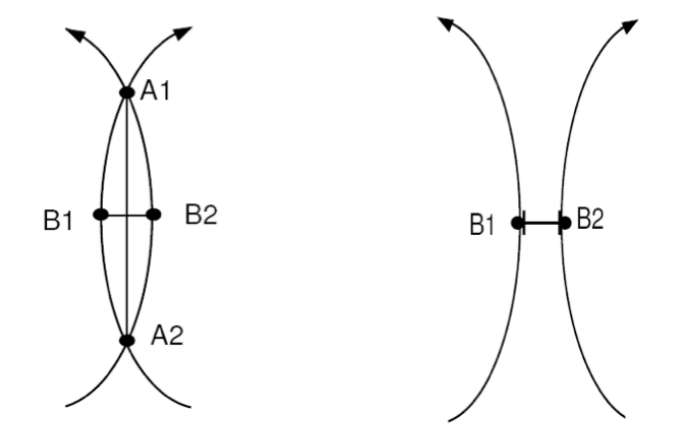
\includegraphics[width=0.45\textwidth]{fig/conversion_diag}
  \caption[Diagram illustrating electron conversion rejection variables]{Diagram
    illustrating the electron conversion rejection variables, \Distnm and
    \DeltaCotThetanm. \Distnm is the distance between points B1 and B2 in the
    $x-y$-plane. Here, the two tracks from the photon conversion are
    parallel. \Distnm is negative when the two tracks overlap and positive
    otherwise~\cite{cms_an_2009_159}.}
  \label{fig:conversion_diag}
\end{figure}

The pseudorapidity acceptance for electrons is $|\eta| < 2.5$. However, the
barrel-endcap transition region, $1.4442 < |\eta| < 1.566$ is explicitly excluded.

\ctable[
caption=Table showing cut values for the simple cut-based electron indentification working points,
label=tbl:reco_electronid
]{lcccccc}{
}{\FL
Efficiency           & 0.95  & 0.9   & 0.85  & 0.8   & 0.7   & 0.6 \ML
\multicolumn{7}{c}{Conversion Rejection}\ML
Missing Hits         & 1     & 1     & 1     & 0     & 0     & 0 \NN
\Dist                & -     & 0.02  & 0.02  & 0.02  & 0.02  & 0.02\NN
\DeltaCotTheta       & -     & 0.02  & 0.02  & 0.02  & 0.02  & 0.02\ML
\multicolumn{7}{c}{Barrel}\ML
Combined Isolation   & 0.15  & 0.1   & 0.09  & 0.07  & 0.04  & 0.03 \NN
\sigmaieta           & 0.01  & 0.01  & 0.01  & 0.01  & 0.01  & 0.01 \NN
\deltaphiin          & 0.8   & 0.8   & 0.06  & 0.06  & 0.03  & 0.025 \NN
\deltaetain          & 0.007 & 0.007 & 0.006 & 0.004 & 0.004 & 0.004 \NN
\HoverE              & 0.15  & 0.12  & 0.04  & 0.04  & 0.025 & 0.025 \ML
\multicolumn{7}{c}{Endcaps}\ML
Combined Isolation   & 0.1   & 0.07  & 0.06  & 0.06  & 0.03  & 0.02 \NN
\sigmaieta           & 0.03  & 0.03  & 0.03  & 0.03  & 0.03  & 0.03 \NN
\deltaphiin          & 0.7   & 0.7   & 0.04  & 0.03  & 0.02  & 0.02 \NN
\deltaetain          & 0.01  & 0.009 & 0.007 & 0.007 & 0.005 & 0.005 \NN
\HoverE              & 0.07  & 0.05  & 0.025 & 0.025 & 0.025 & 0.025 \LL
}

\fig~\ref{fig:reco_ele_perf} shows the \ac{ECAL} energy resolution as
a function of electron energy from the results of a beam test. The
electron fake rate is shown as a function of \Et and $\eta$ for the
95\% and 80\% efficiency working points in
\fig~\ref{fig:reco_ele_fake_rate}.

\begin{figure}
  \centering
  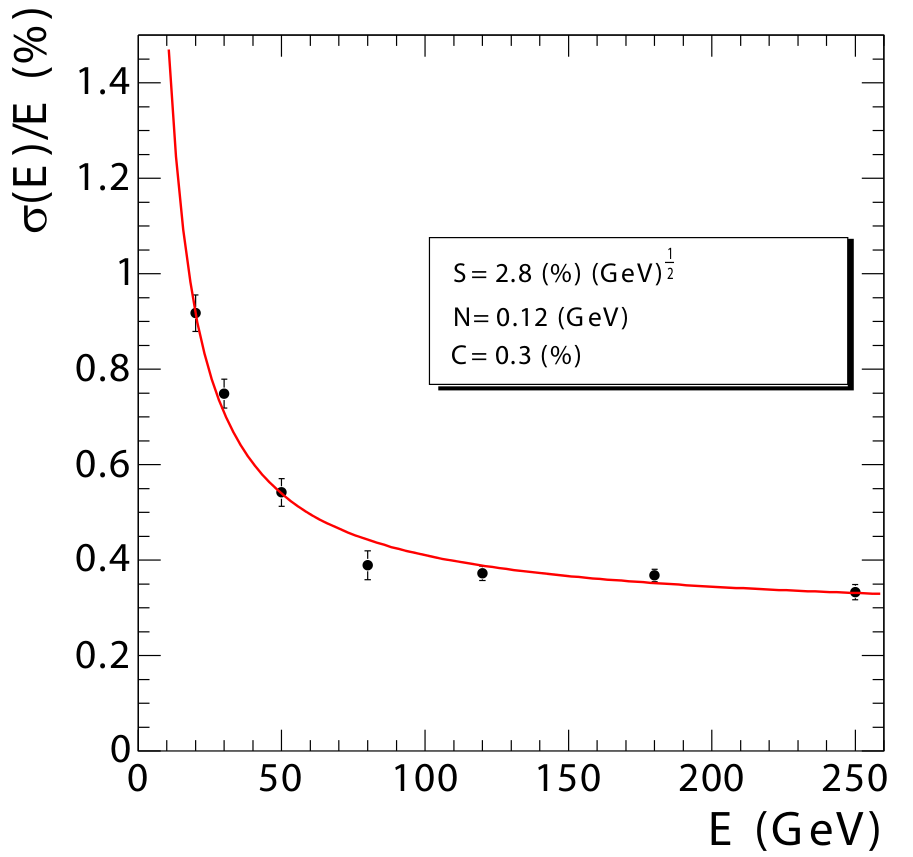
\includegraphics[width=0.6\textwidth]{fig/ele_perf}
  \caption[\ac{ECAL} energy resolution]{\ac{ECAL} energy
    resolution as a function of electron energy from the results of a
    test beam measurement. The energy has been measured in an array of
    $3\times 3$ crystals with an electron impacting the central
    crystal. The values of the stochastic ($S$), noise ($N$) and
    constant ($C$) terms are also shown~\cite{cms_jinst}.}
  \label{fig:reco_ele_perf}
\end{figure}

\begin{figure}
\centering
\subfloat[Barrel]{\label{fig:reco_ele_fake_rate_a}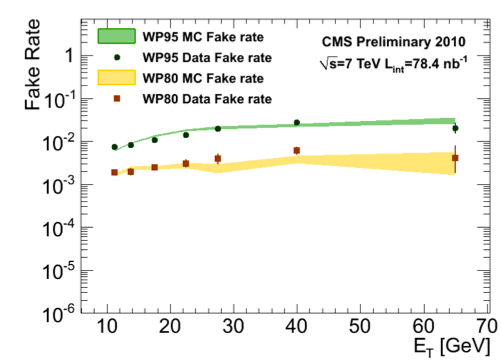
\includegraphics[width=0.45\textwidth]{fig/ele_fake_rate_a}}\quad
\subfloat[Endcap]{\label{fig:reco_ele_fake_rate_b}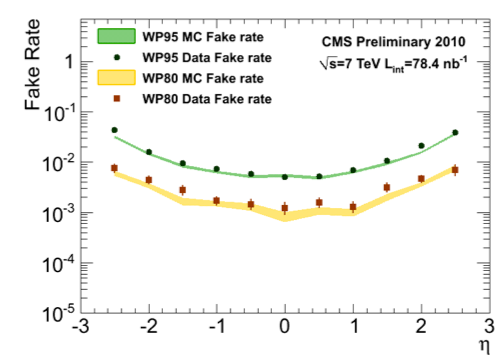
\includegraphics[width=0.45\textwidth]{fig/ele_fake_rate_b}}
\caption[Electron fake rate for 95\% and 80\% efficiency working points]{Electron fake rate per reconstructed electron as a function
  of \subref{fig:reco_ele_fake_rate_a} \Et and
  \subref{fig:reco_ele_fake_rate_b} $\eta$ for the 95\% and 80\%
  efficiency working points. Results are shown for data and
  \ac{MC}~\cite{cms_ele_reco_pas}.}
\label{fig:reco_ele_fake_rate}
\end{figure}

\section{Jets}
\label{sec:reco_jets}
Four types of jets are reconstructed at \ac{CMS}: \acf{Calo} jets, \ac{PF} jets,
\ac{JPT} jets and track jets~\cite{jet_perf_pas}. \ac{Calo} jets are
reconstructed from energy deposits in the \ac{ECAL} and \ac{HCAL}, combined into
\emph{calorimeter towers}. Calorimeter towers consist of one or more \ac{HCAL} cells
with geometrically matched \ac{ECAL} crystals. Electronics noise is suppressed
by applying a threshold to the calorimeter cells, with pile-up effects reduced
by a requirement placed on the tower energy.

\ac{JPT} jets associate tracks with \ac{Calo} jets -- using the tracker to give
enhanced \Pt resolution and response. \ac{PF} jets are products of the \acl{PF}
algorithm described in \sec~\ref{sec:reco_pf}. Finally, track jets are
reconstructed from well measured tracks in the central tracker. Jets are
clustered using the \antiKT algorithm~\cite{antiKT} with a size parameter,
$R=0.5$.

A useful jet-derived quantity is the ``transverse hadronic energy'' or \HT. This
is simply defined as the scalar sum of the transverse momentum of jets in the
event. The jets considered will be selected according to some quality and
acceptance criteria.

\subsection{Jet Energy Corrections and \acl{JES}}
In general, the jet energy -- as measured in the calorimeters -- will be
different from the corresponding particle jet energy. In order to correct for
this difference, jet energy corrections are
applied~\cite{jet_energy_cms,jet_energy_pas}. The calibration of the jet energy
will be referred to as the \acf{JES}.

At \ac{CMS}, jet energy corrections have been been factorised into three parts:
\begin{itemize}
\item \emph{offset corrections} remove excess energy due to electronics noise
  and pile-up;
\item \emph{relative corrections} attempt to remove variations in jet response
  with respect to pseudorapidity and
\item \emph{absolute corrections} attempt to remove variations in jet response
  with respect to \Pt.
\end{itemize}

These are measured using a variety of techniques, including the balancing of
dijets, \gammajets and \Zjets events. \fig~\ref{fig:reco_jet_energy_corr} shows
the total corrections factor as a function of $\eta$, for two values of the jet
\Pt. With these corrections applied, the residual uncertainty on the \ac{JES}
has been evaluated as a function of jet $\eta$ and \Pt. This will turn out to be
a significant source of systematic uncertainty for the analyses presented in
\chaps~\ref{sec:wpol}~and~\ref{sec:susysearch}.

\begin{figure}[h!]
  \centering
  \subfloat[\unit{50}{\GeV}]{\label{fig:jet_energy_corr_50}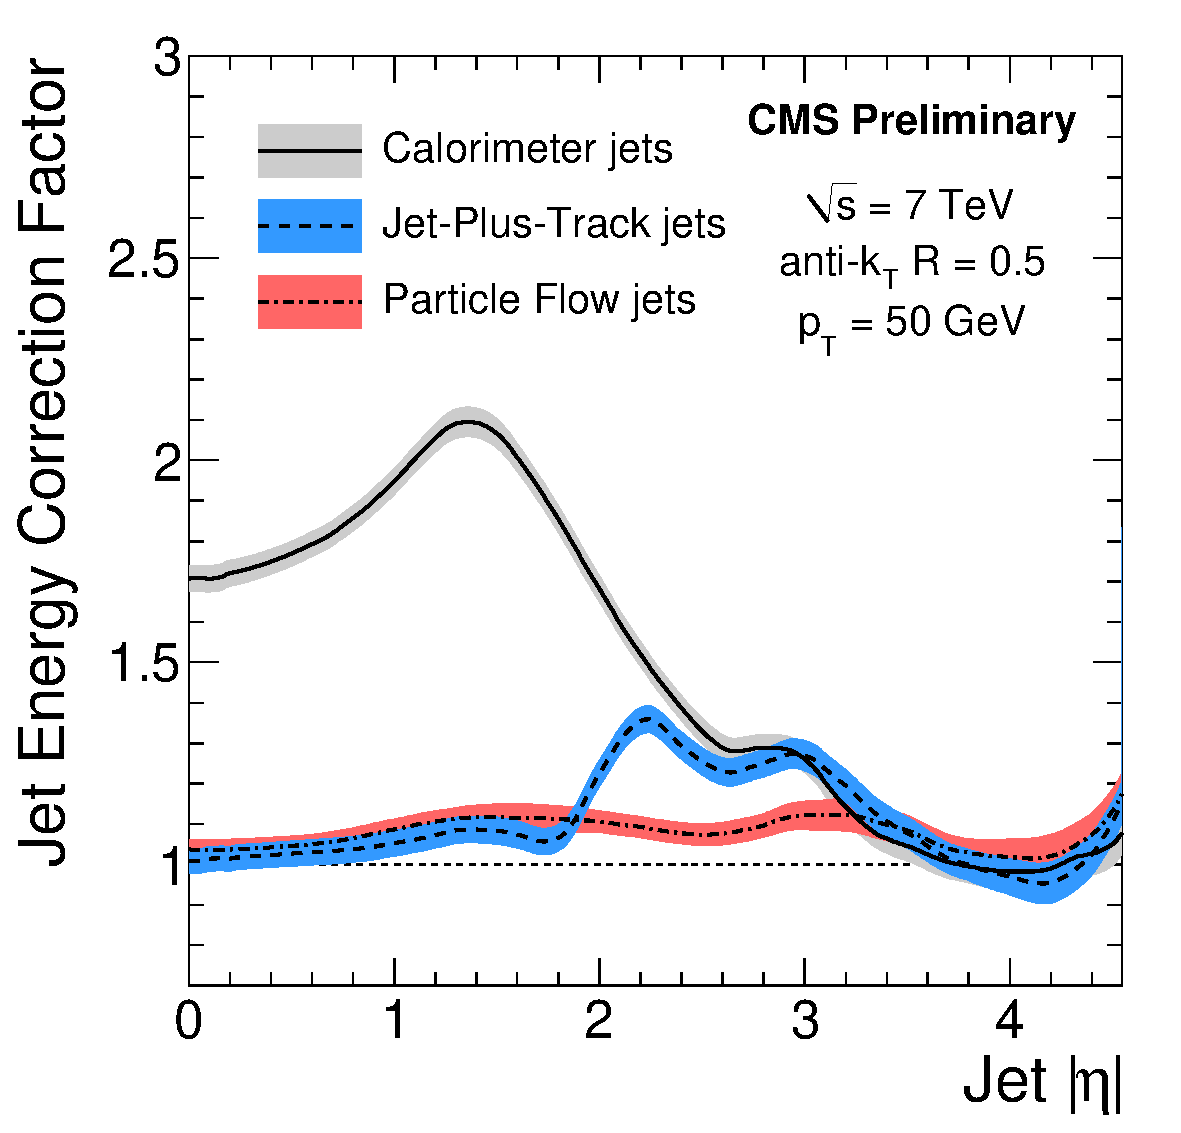
\includegraphics[width=0.45\textwidth]{fig/jet_energy_corr_pt50.pdf}}\quad
  \subfloat[\unit{200}{\GeV}]{\label{fig:jet_energy_corr_200}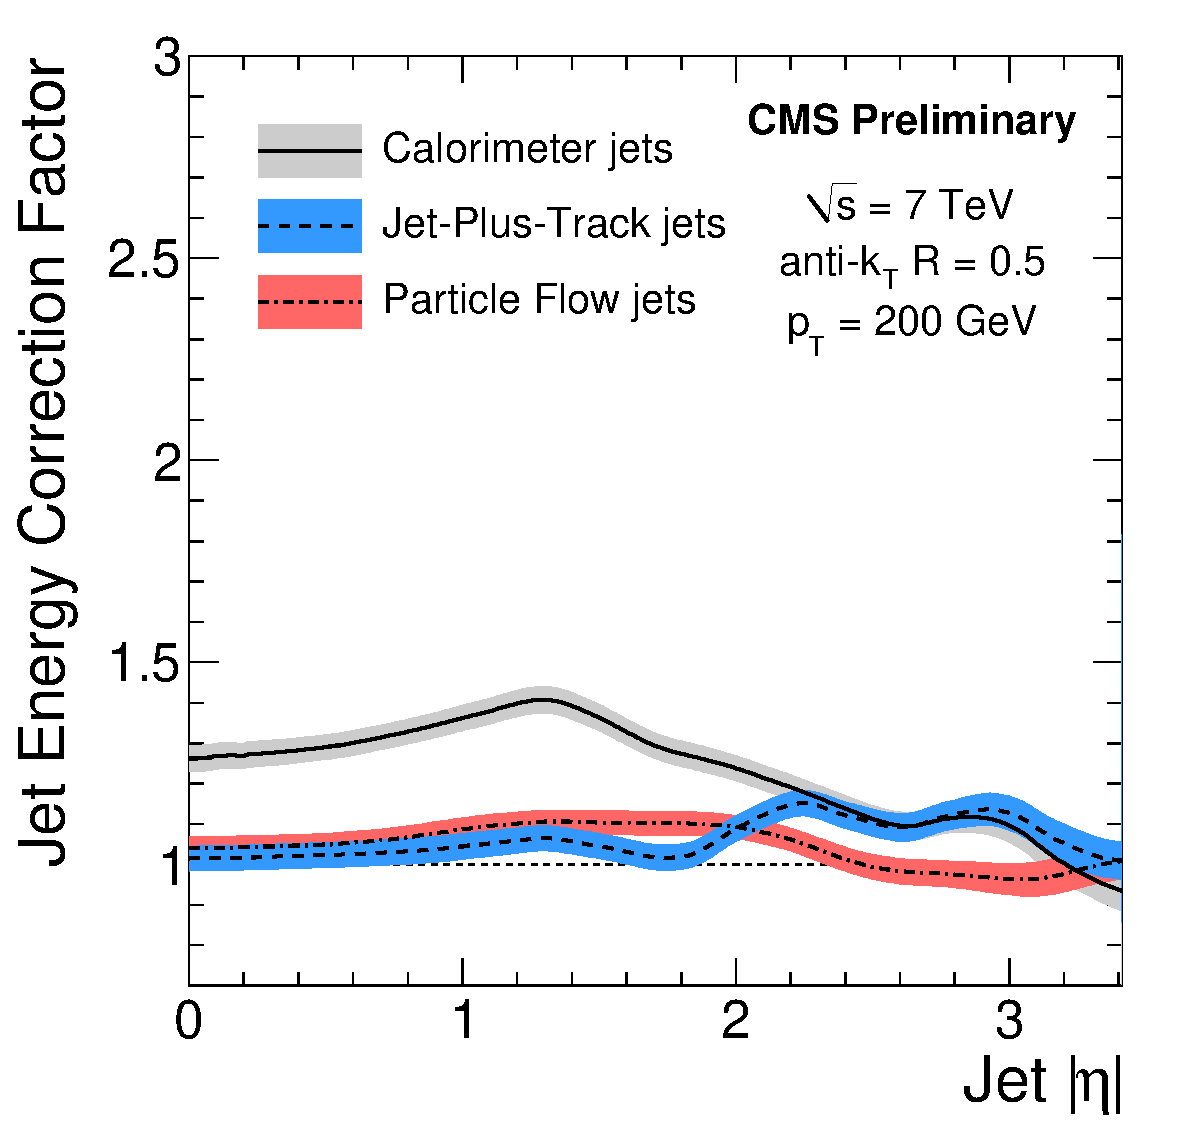
\includegraphics[width=0.45\textwidth]{fig/jet_energy_corr_pt200.pdf}}\quad
  \caption[Total jet energy correction factor as a function of $\eta$]{Total jet
    energy correction factor as a function of $\eta$ for jets with transverse
    momenta of \subref{fig:jet_energy_corr_50} \unit{50}{\GeV} and
    \subref{fig:jet_energy_corr_200} \unit{200}{\GeV}. Corrections are shown for
    \ac{Calo}, \ac{JPT} and \ac{PF} jets separately. The bands indicate the
    corresponding uncertainties~\cite{jet_energy_pas}.}
  \label{fig:reco_jet_energy_corr}
\end{figure}

\section{Missing Energy}
\label{sec:reco_missing_energy}
Certain particles, such as neutrinos, are not reconstructed by the \ac{CMS}
detector. However, their presence may be inferred by considering the total
momentum of particles reconstructed by the detector and comparing this with the
momentum of the initial state. Any imbalance in these quantities can be
attributed to the presence of some ``invisible'' particles -- a \emph{missing
  energy} signature.

At a hadron collider, the situation is complicated by the fact that the boost of
the initial partons parallel to the beam-line is not known. Hence missing energy
measurement along this axis is not possible. For this reason, transverse
quantities are used instead -- most commonly the \emph{missing transverse
  energy}, \METv. This can be defined generically as
\begin{equation*}
\METv = -\sum_{o \in \textrm{objects}} \vec{p}_T^o,
\end{equation*}
where $p_T^o$ represents the transverse momentum of object, $o$. The choice of a
suitable set of objects then leads to a number of alternative definitions of
\METv. The magnitude of this quantity, often used in event selection, will be
denoted \MET. Similar notation will be used for other transverse vector
quantities.

At \ac{CMS}, the simplest measurement of \METv is \emph{\ac{Calo} \METv} which
sums over the calorimeter tower energies (\ac{ECAL} and \ac{HCAL}).  An energy
threshold is applied to the towers in order to reject electronics
noise. Alternatively, \emph{\ac{PF} \METv} sums over the candidate particles output by
the \ac{PF} algorithm. This will be discussed further in
\sec~\ref{sec:reco_pf}. As will be seen, this provides the most sensitive \METv
measurement at \ac{CMS} and thus is used throughout the following analysis
work. It should be assumed, unless otherwise noted, that references to \METv or
derived quantities make use of the \ac{PF} measurement.

Alternative missing energy quantities can be defined for other purposes. The
\emph{missing transverse hadronic energy}, \MHT, is formed by taking the vector
sum,
\begin{equation*}
\MHTv = -\sum_{j \in \textrm{jets}} \vec{E_T^j}.
\end{equation*}
This is used to measure the transverse energy of particles recoiling against the
jets in an event. For example, in \Wjets events, the recoiling system is the \PW
boson. \MHTv is therefore one possible measurement of the \PW boson transverse
momentum, \PtWv.


\section{Particle Flow at \acs{CMS}}
\label{sec:reco_pf}
The \ac{PF} algorithm~\cite{cms_pf_pas,cms_pf_pas2} attempts to provide a
global reconstruction of the event -- accurate determination of the type, energy
and direction of all stable particles -- by combining measurements from all
subdetectors in \ac{CMS}. This strategy is well suited for use with the \ac{CMS}
detector. The silicon tracker is able to reconstruct charged particle tracks
with high efficiency and purity, down to transverse momenta as low as
\unit{150}{\MeV}. Additionally, the granularity of the \ac{ECAL} is sufficient
for the separation of photons and charged particle energy deposits in jets with
\Pt of a few hundred \GeV~\cite{cms_pf_pas}. In contrast, the \ac{HCAL} is much
coarser. However, the combined energy resolution of both calorimeters is $\sim
10\%$ at \unit{100}{\GeV}. This allows identification of the energy deposits
associated with neutral hadrons as an excess on top of that accounted for by
matching the deposits with charged tracks. The \ac{PF} algorithm is able to
reconstruct the components of jets and hadronic tau decays -- primarily charged
hadrons, neutral hadrons and photons. This provides an improved measurement of
the jet energy and thus also of \METv.

The particle flow algorithm proceeds by linking tracks and energy clusters to
form ``blocks''. An event display which illustrates this process is shown in
\fig~\ref{fig:reco_pf_diag}. A single block may contain a combination of a
charged particle track, one or more energy clusters and a muon. The fine
granularity of the \ac{CMS} detector ensures that blocks typically contain 1, 2
or 3 elements.  The links between each block are parameterised by a ``distance''
which encodes the quality of the link. Advanced tracking and calorimeter
clustering algorithms have been developed to meet the needs of \ac{PF}
reconstruction. These will be discussed in the following sections.

\begin{figure}[h!]
\centering
\subfloat[]{\label{fig:reco_pf_diag1}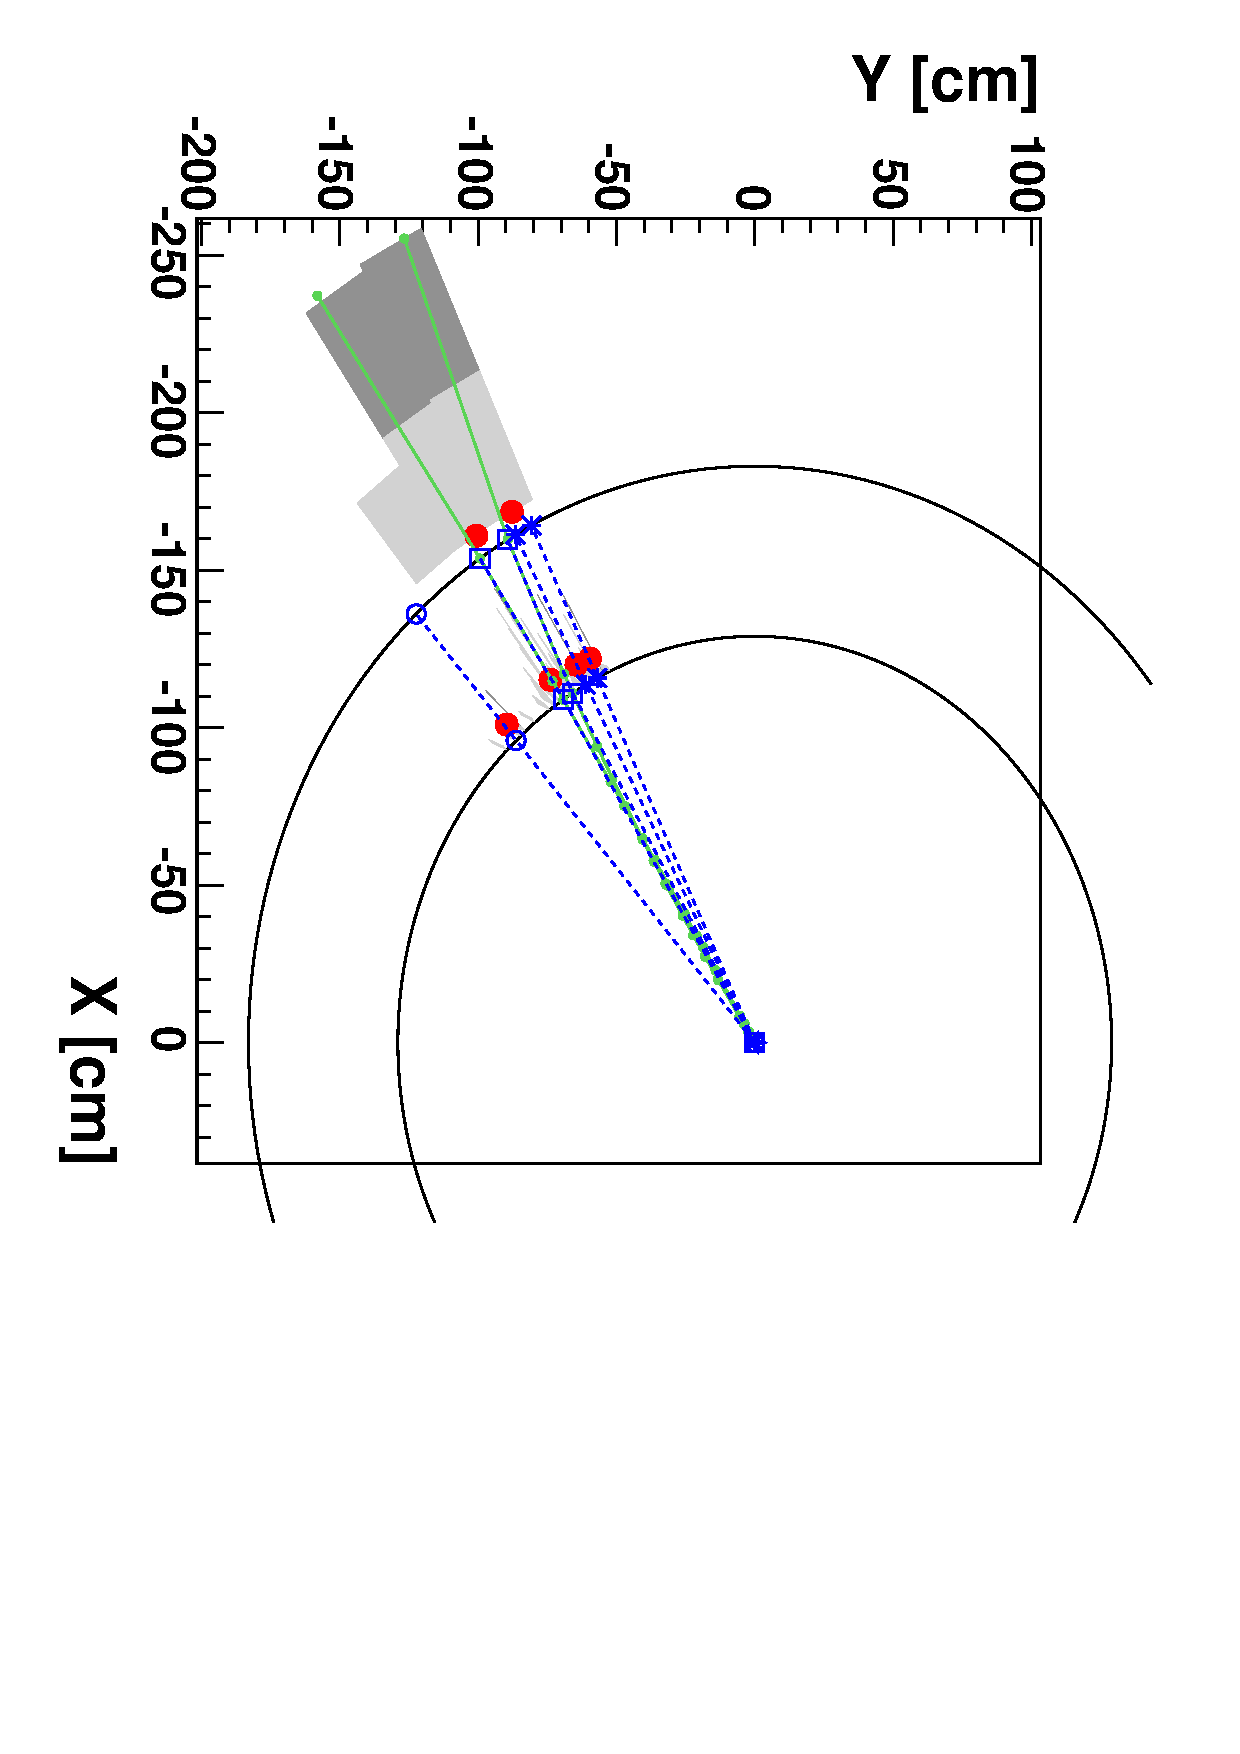
\includegraphics[width=0.5\textwidth]{fig/pf_diag1}}\\
\subfloat[]{\label{fig:reco_pf_diag2}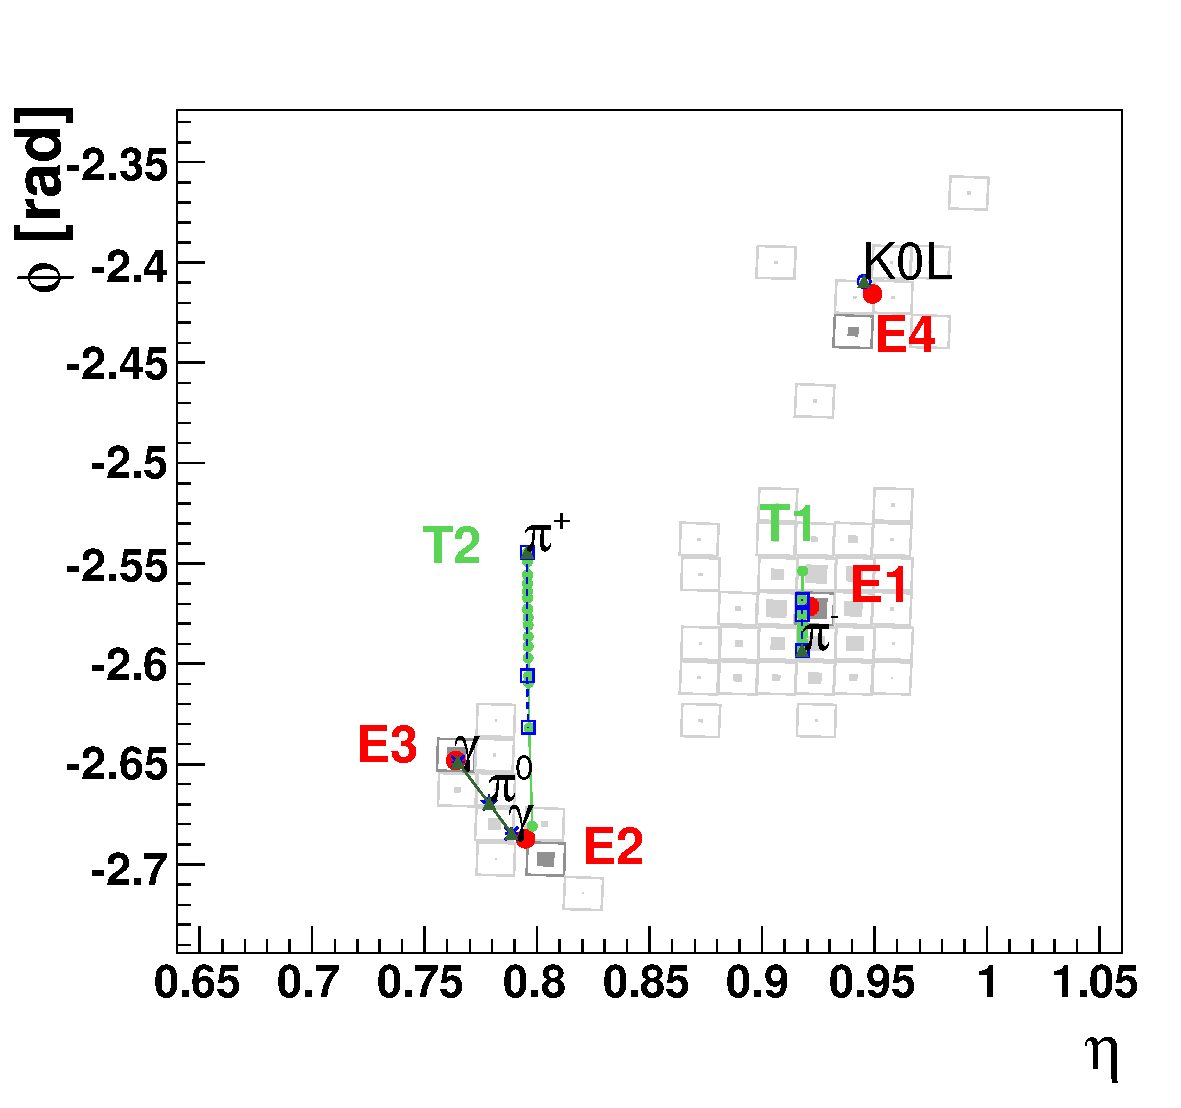
\includegraphics[width=0.4\textwidth]{fig/pf_diag2}}\quad
\subfloat[]{\label{fig:reco_pf_diag3}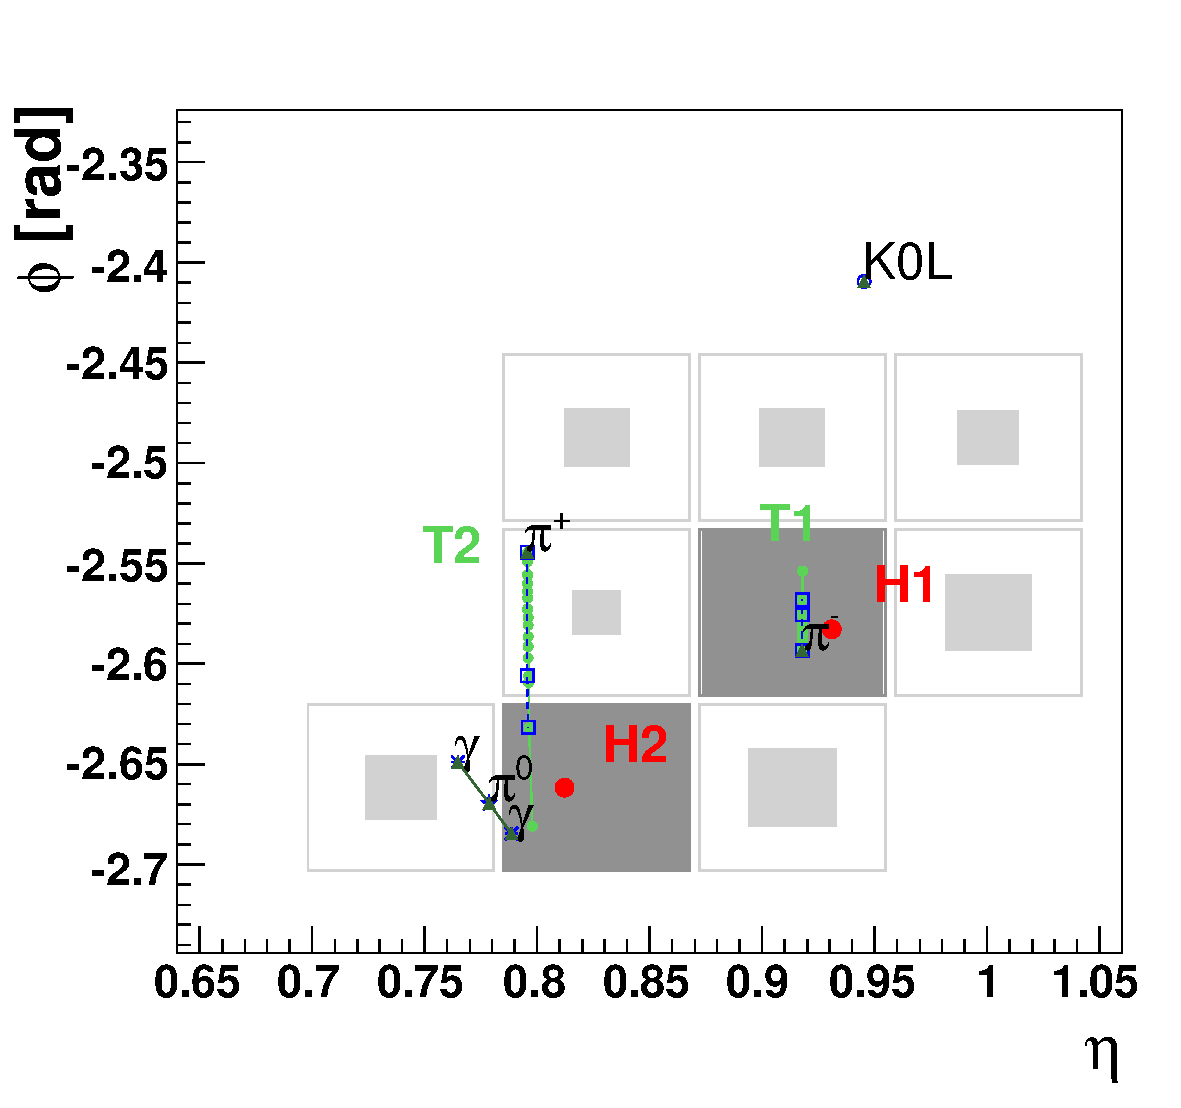
\includegraphics[width=0.4\textwidth]{fig/pf_diag3}}
\caption[\acl{PF} event display showing a hadronic jet]{An event display showing
  a hadronic jet in~\subref{fig:reco_pf_diag1} the $(x,y)$-plane,
  \subref{fig:reco_pf_diag2} an $(\eta,\phi)$ view at the surface of the
  \ac{ECAL} and~\subref{fig:reco_pf_diag3} the same orientation at the surface
  of the \ac{HCAL}. These two surfaces appear as circular arcs
  in~\subref{fig:reco_pf_diag1}. The \PKlong, \Ppiminus, \Ppiplus, \Ppizero and
  the two photons from its decay are shown. The \PKlong, \Ppiminus and two
  photons result in clear, well-separated \ac{ECAL} clusters -- round points
  labelled E1 to E4~\subref{fig:reco_pf_diag2}. The \Ppiplus and \Ppiminus are
  reconstructed as charged tracks -- green lines labelled T1 and T2 -- which
  point to the two \ac{HCAL} clusters -- round points labelled H1 and
  H2~\cite{cms_pf_pas}.}
\label{fig:reco_pf_diag}
\end{figure}

\subsection{Iterative Tracking}
The tracker provides far superior measurements of the momentum and direction of
charged hadrons than is possible with the calorimeters. It is important
therefore that the tracks, which form the input to the \ac{PF} procedure, be
reconstructed with near 100\% efficiency. The fake rate must also be low to
avoid excess energy counting.

To meet these requirements, tracks are reconstructed using an iterative
algorithm. This begins by reconstructing tracks with very tight selection
requirements. Hits which can be unambiguously assigned in this step are then
removed from consideration. The algorithm is iterated, and reconstruction of
tracks from the remaining hits is attempted, this time with loosened selection
criteria. This procedure is repeated with progressively looser selection
criteria. This ensures high efficiency, whilst the removal of hits at each stage
reduces the fake rate induced by combinatorics.  After three iterations, tracks
originating close to the beam line are reconstructed with an efficiency of
99.5\% for muons and $>90\%$ for charged hadrons. The fourth and fifth
iterations relax constraints on the vertex, allowing the reconstruction of
secondary charged particles.

\subsection{Calorimeter Clustering}
The success of the \ac{PF} reconstruction also depends on certain aspects of the
energy-clustering algorithm. In particular, as for the tracks, the clustering
must be highly efficient and able to distinguish closely-spaced energy deposits.
To this end, a specialised clustering algorithm was developed. This algorithm is
used in the \ac{ECAL}, \ac{HCAL} and \ac{PS} but not in the \ac{HF}, where each
cell is treated as a single cluster.

The first step of the algorithm produces \emph{seed clusters}. These are local
maxima in the calorimeter cell energies which have passed a minimum threshold
requirement.  These seed clusters are then extended to include cells sharing at
least one side in common with a cell already in the cluster and an energy exceeding a
threshold chosen according to the standard deviation of electronics noise in the
calorimeter. These \emph{topological clusters} are then transformed into
\emph{particle flow clusters}, with a separate particle flow cluster for each
seed within the topological cluster. The energy and position of each particle
flow cluster is determined iteratively, with the energy of each cell shared
among the particle flow clusters.

\subsection{Building Links}
Each track is extrapolated from the position of its last measured hit to: the
\ac{PS}, the \ac{ECAL} at a depth corresponding to the expected maximum for an
electron shower and the \ac{HCAL} at a depth of 1 interaction length. In each
case, if the extrapolated track position lies within the envelope of a cluster,
a link is created. The link distance is the $(\eta, \phi)$ distance between the
extrapolated track and the cluster. The envelope may be enlarged with respect to
the cluster by the extent of a single cell.

Energy contributions from bremsstrahlung photons are included by extrapolating
the track-tangent at each tracker layer to the \ac{ECAL}. If the extrapolated
track lies within the envelope of the cluster, a link is created.  Links are
also created between calorimeter clusters in different subdetectors if the
cluster position in the finer-grained calorimeter lies within the envelope of
the more coarsely grained calorimeter. The link distance is taken to be the
$(\eta, \phi)$ separation of the two clusters.

Muons are included when a global fit between a track in the tracker and a muon
track in the muon chambers yields an acceptable \chisq. If several global muons
are found for a single muon track, only that possessing the smallest \chisq is
retained -- with the link distance determined by the \chisq.

\subsection{Particle Reconstruction}
In the first stage, muons are reconstructed. Each global muon gives rise to a
particle flow muon, providing that its momentum, as determined from the global
fit, is compatible with the track momentum to within 3 standard deviations. The
corresponding track is then removed from the block.

The next step is electron reconstruction. Electron tracks in the block are first
selected by a pre-identification step. This exploits the fact that electrons
often leave short tracks and lose energy via bremsstrahlung. Pre-identified
electrons are then refit with a \ac{GSF} (see \sec~\ref{sec:reco_electrons}) and
projected into the \ac{ECAL}.  Candidates passing tracking and calorimetric
criteria are reconstructed as particle flow electrons. The track and associated
\ac{ECAL} clusters are then removed from the block.

Tracks remaining are then subjected to a tighter set of quality requirements, in
particular that the track \Pt uncertainty be smaller than the relative
calorimeter energy resolution for a charged hadron. Whilst some real hadrons are
lost by this requirement, the energy will be retained in the more accurate
measurement from the calorimeter.

Reconstruction of photons and neutral hadrons involves comparison of the track
momentum to the calorimetric energy. The cluster energies in the \ac{ECAL} are
calibrated for photons and in the \ac{HCAL}, for \unit{50}{\GeV} pions. For the
comparison to be valid, these must be re-calibrated to account for
non-linearities in the \ac{HCAL}, as well as the differing response of the
\ac{ECAL} to hadrons.

In the case that several tracks are linked to a single \ac{HCAL} cluster, the
total momentum of the tracks is compared to the calibrated calorimetric energy.
Tracks linked to multiple clusters are resolved by preserving the closest link
or in certain cases, links. The track momentum is then compared to the total
calibrated calorimetric energy.

In the rare case that the energy is smaller than the track momentum by more than
three standard deviations, a relaxed search for fake tracks and global muons is
initiated. Global muons are identified as \ac{PF} muons if their momentum is
measured with an uncertainty below 25\%. Tracks are then progressively removed
from the block, those with largest momentum uncertainty first, until either all
tracks with an uncertainty $>\unit{1}{\GeV}$ have been considered or the total
track momentum has decreased below the calorimetric energy. The remaining tracks
are interpreted as charged hadrons with momentum and energy measurements taken
from the track momentum, assuming the charged pion mass hypothesis. If the
calorimeter energy and track momentum are compatible within their uncertainties,
the momentum is redefined by a fit of the measurements in the tracker and the
calorimeters. This is helpful at very high energies, where the track parameters
may be less well measured.

In the case that the calibrated energy is greater than the total track momentum
by more than the calorimetric energy resolution, the excess is interpreted as a
photon and possibly a neutral hadron. If the excess is greater than the
\ac{ECAL} energy, a photon is created with this energy and the rest of the
excess interpreted as a neutral hadron. Otherwise, only a photon is
reconstructed from the uncalibrated \ac{ECAL} energy. This stems from the
observation that photons carry 25\% of the energy of a jet, and neutral hadrons
leave only 3\% of the jet energy in the \ac{ECAL}.

Remaining \ac{ECAL} and \ac{HCAL} clusters not linked to a track (or for which
the associated track was disabled in the previous steps) are reconstructed as
photons and neutral hadrons respectively.

\ac{PF} jets are then reconstructed by applying the \antikT algorithm to the
full set of \ac{PF} objects.

\subsection{Physics Performance}
Two aspects of the performance of the \ac{PF} reconstruction are of relevance to
the analysis description that will follow: measurement of \METv and jet
reconstruction. \fig~\ref{fig:reco_pf_jet_energyres} shows a comparison of the
jet energy resolution of \ac{PF} and \ac{Calo} jets as a function of jet
\Pt. The angular resolution is compared in
\fig~\ref{fig:reco_pf_jet_angularres}. The improvement given by the \ac{PF}
algorithm can be clearly seen, particularly at low jet momentum. A similar
comparison of the \MET resolution can be seen in
\fig~\ref{fig:reco_pf_met_res}. Again, the \ac{PF} algorithm is seen to offer
significantly improved resolution.

\begin{figure}[htbp!]
\centering
\subfloat[Barrel]{\label{fig:reco_pf_jet_energyres_barrel}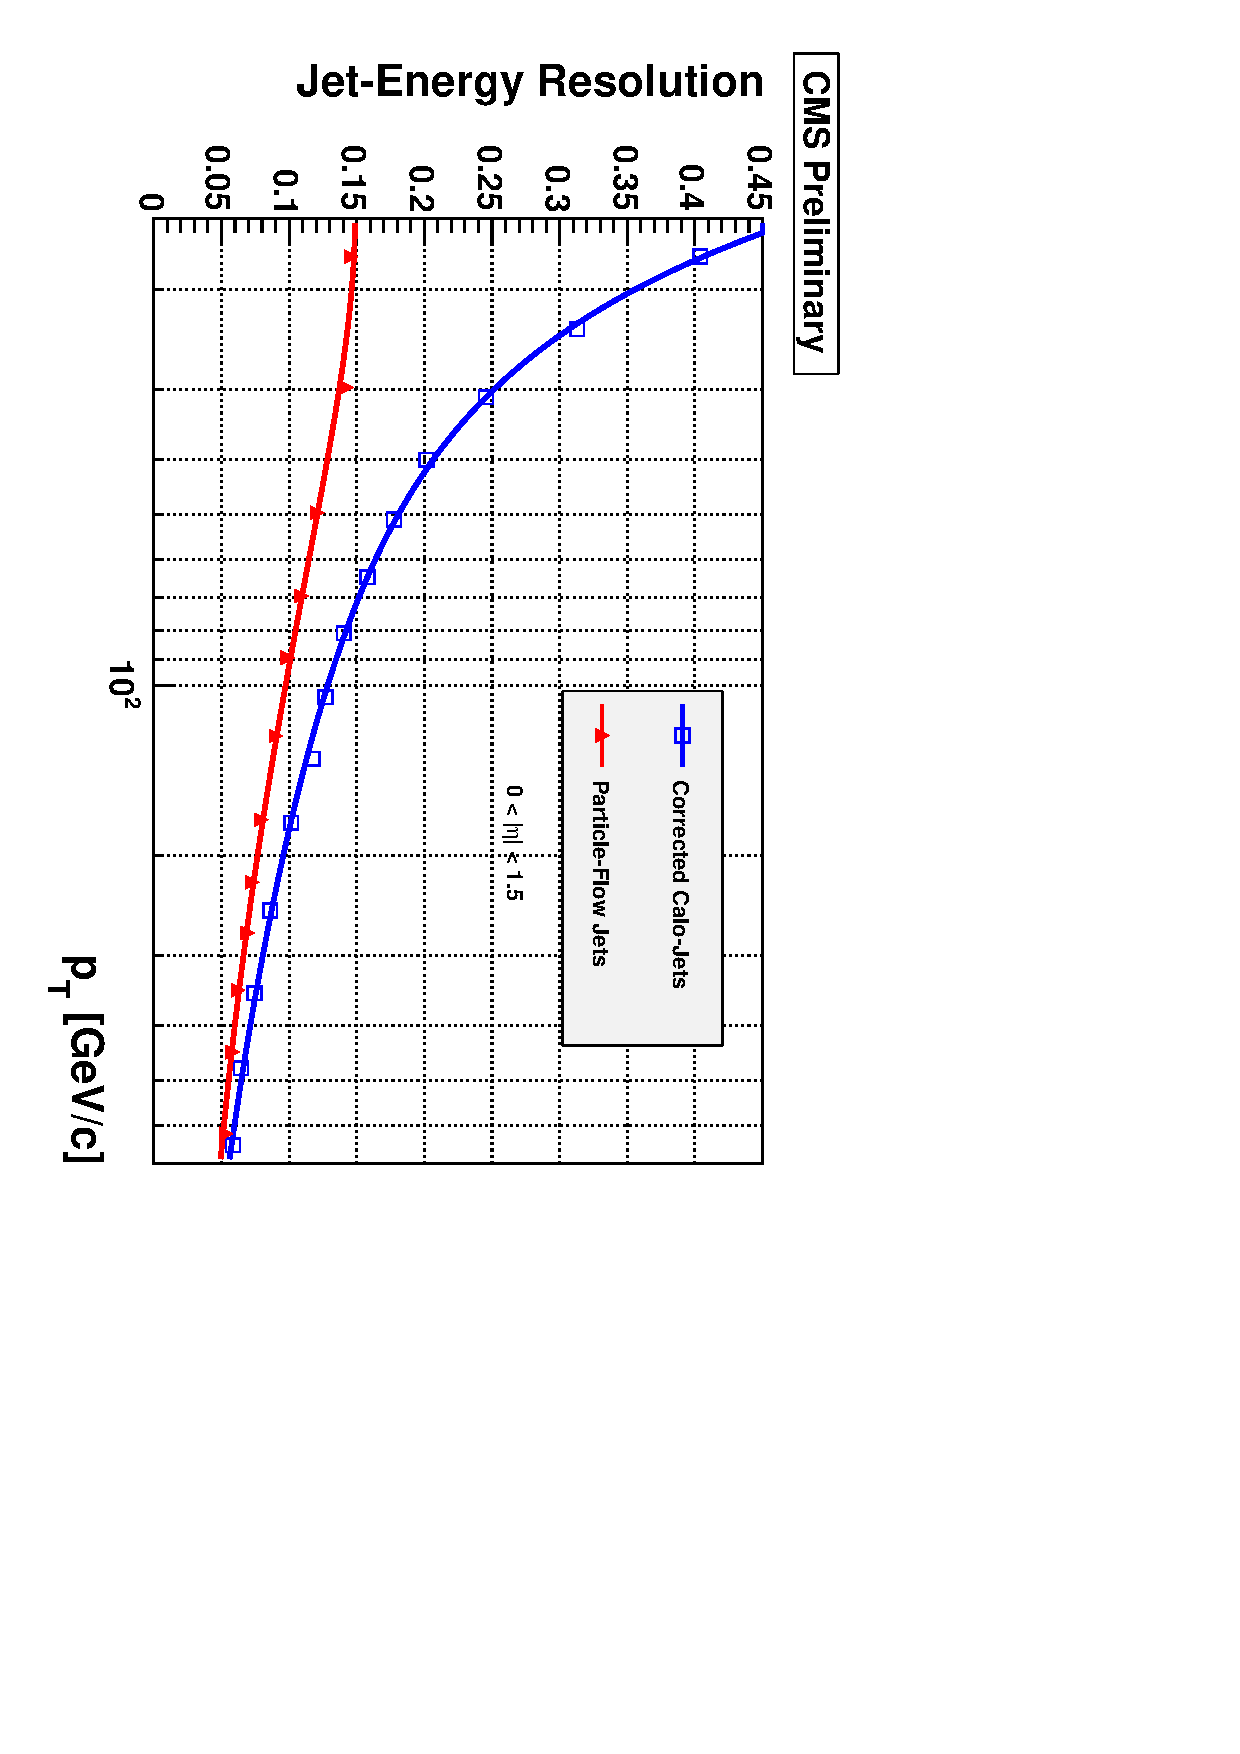
\includegraphics[width=0.45\textwidth]{fig/pf_jet_energyres_barrel}}\quad
\subfloat[Endcap]{\label{fig:reco_pf_jet_energyres_endcap}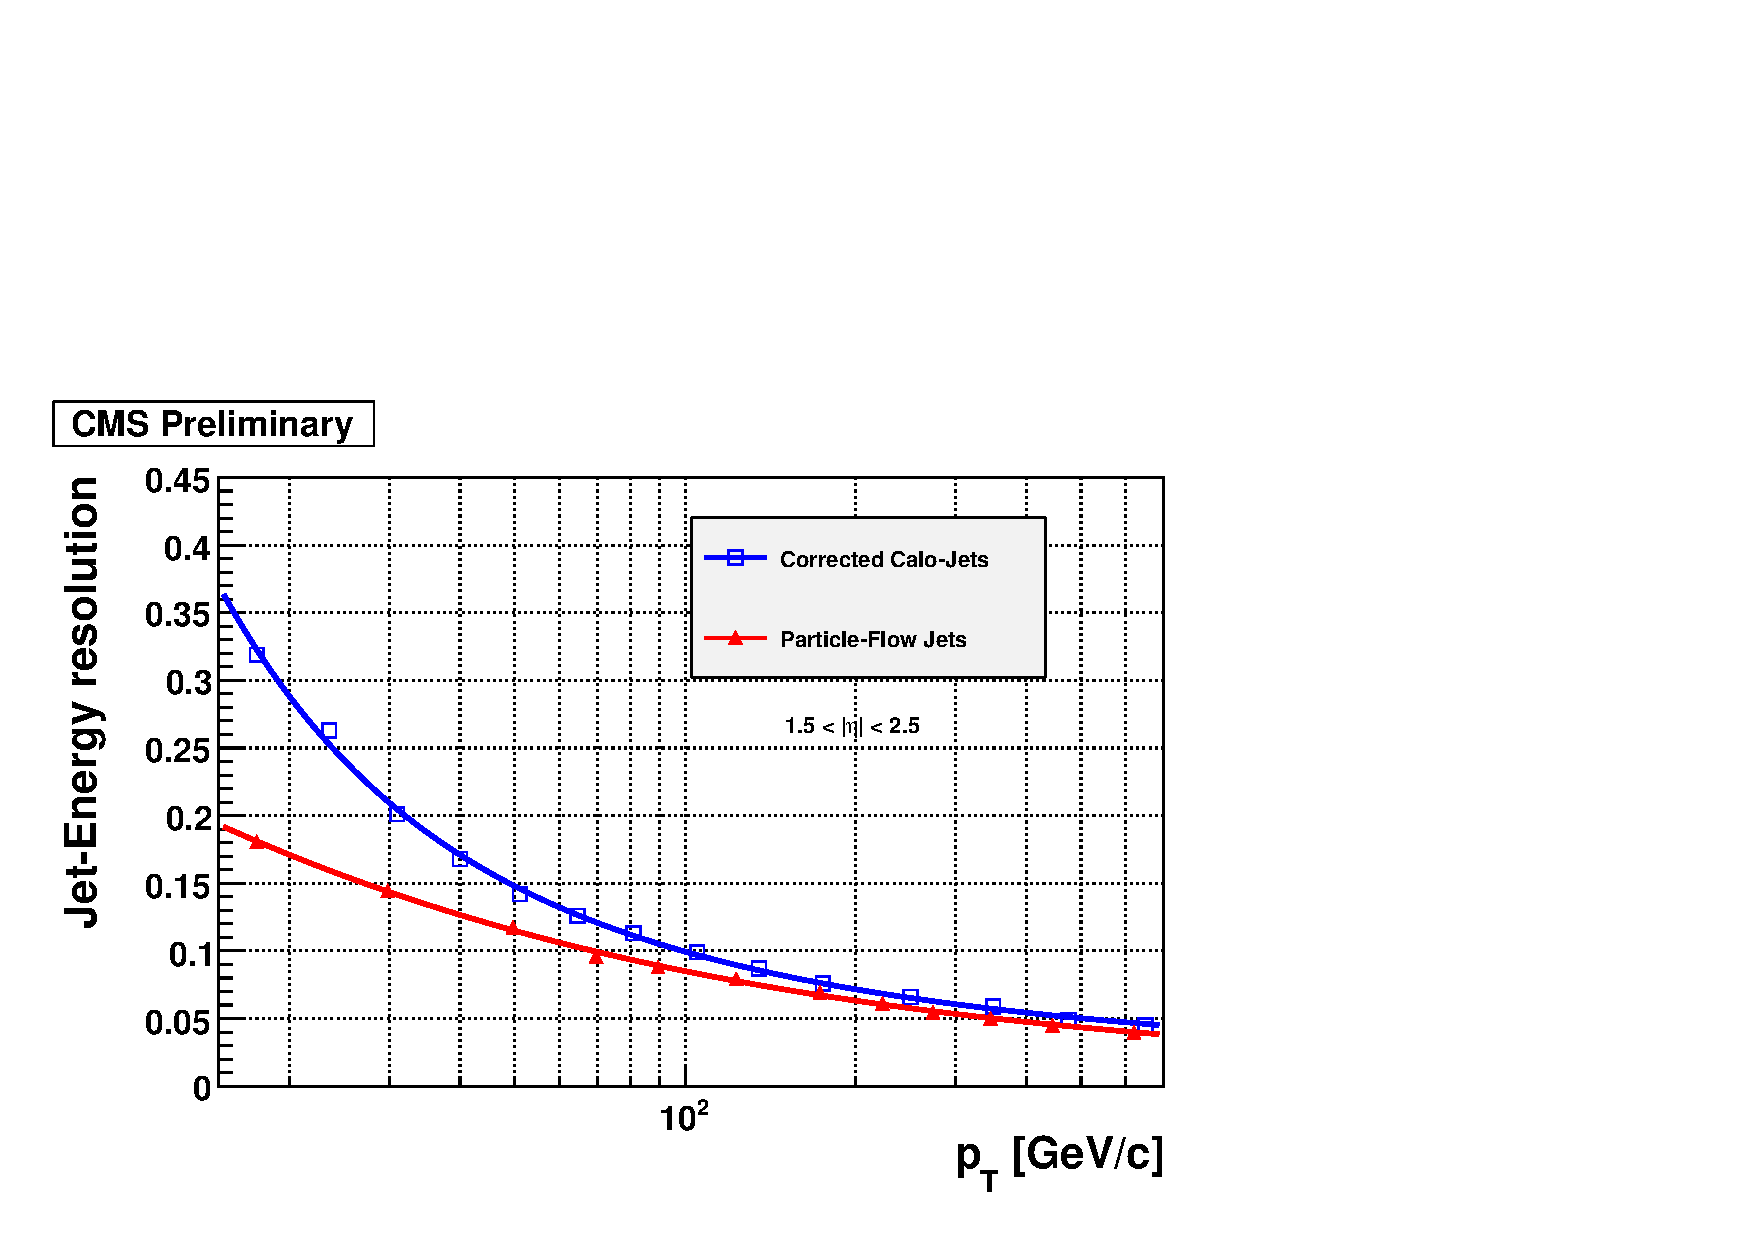
\includegraphics[width=0.45\textwidth]{fig/pf_jet_energyres_endcap}}\quad
\caption[Jet energy resolution as a function of \Pt]{Jet energy resolution as a
  function of \Pt for the \subref{fig:reco_pf_jet_energyres_barrel} barrel and
  \subref{fig:reco_pf_jet_energyres_endcap} endcap. Calo-jet values are
  displayed as open squares and \ac{PF} jet as upwards triangles. The curves are
  fit to the sum of a constant term, a stochastic term and a noise term~\cite{cms_pf_pas}.}
\label{fig:reco_pf_jet_energyres}
\end{figure}

\begin{figure}[htbp!]
\centering
\subfloat[$\eta$]{\label{fig:reco_pf_jet_etares}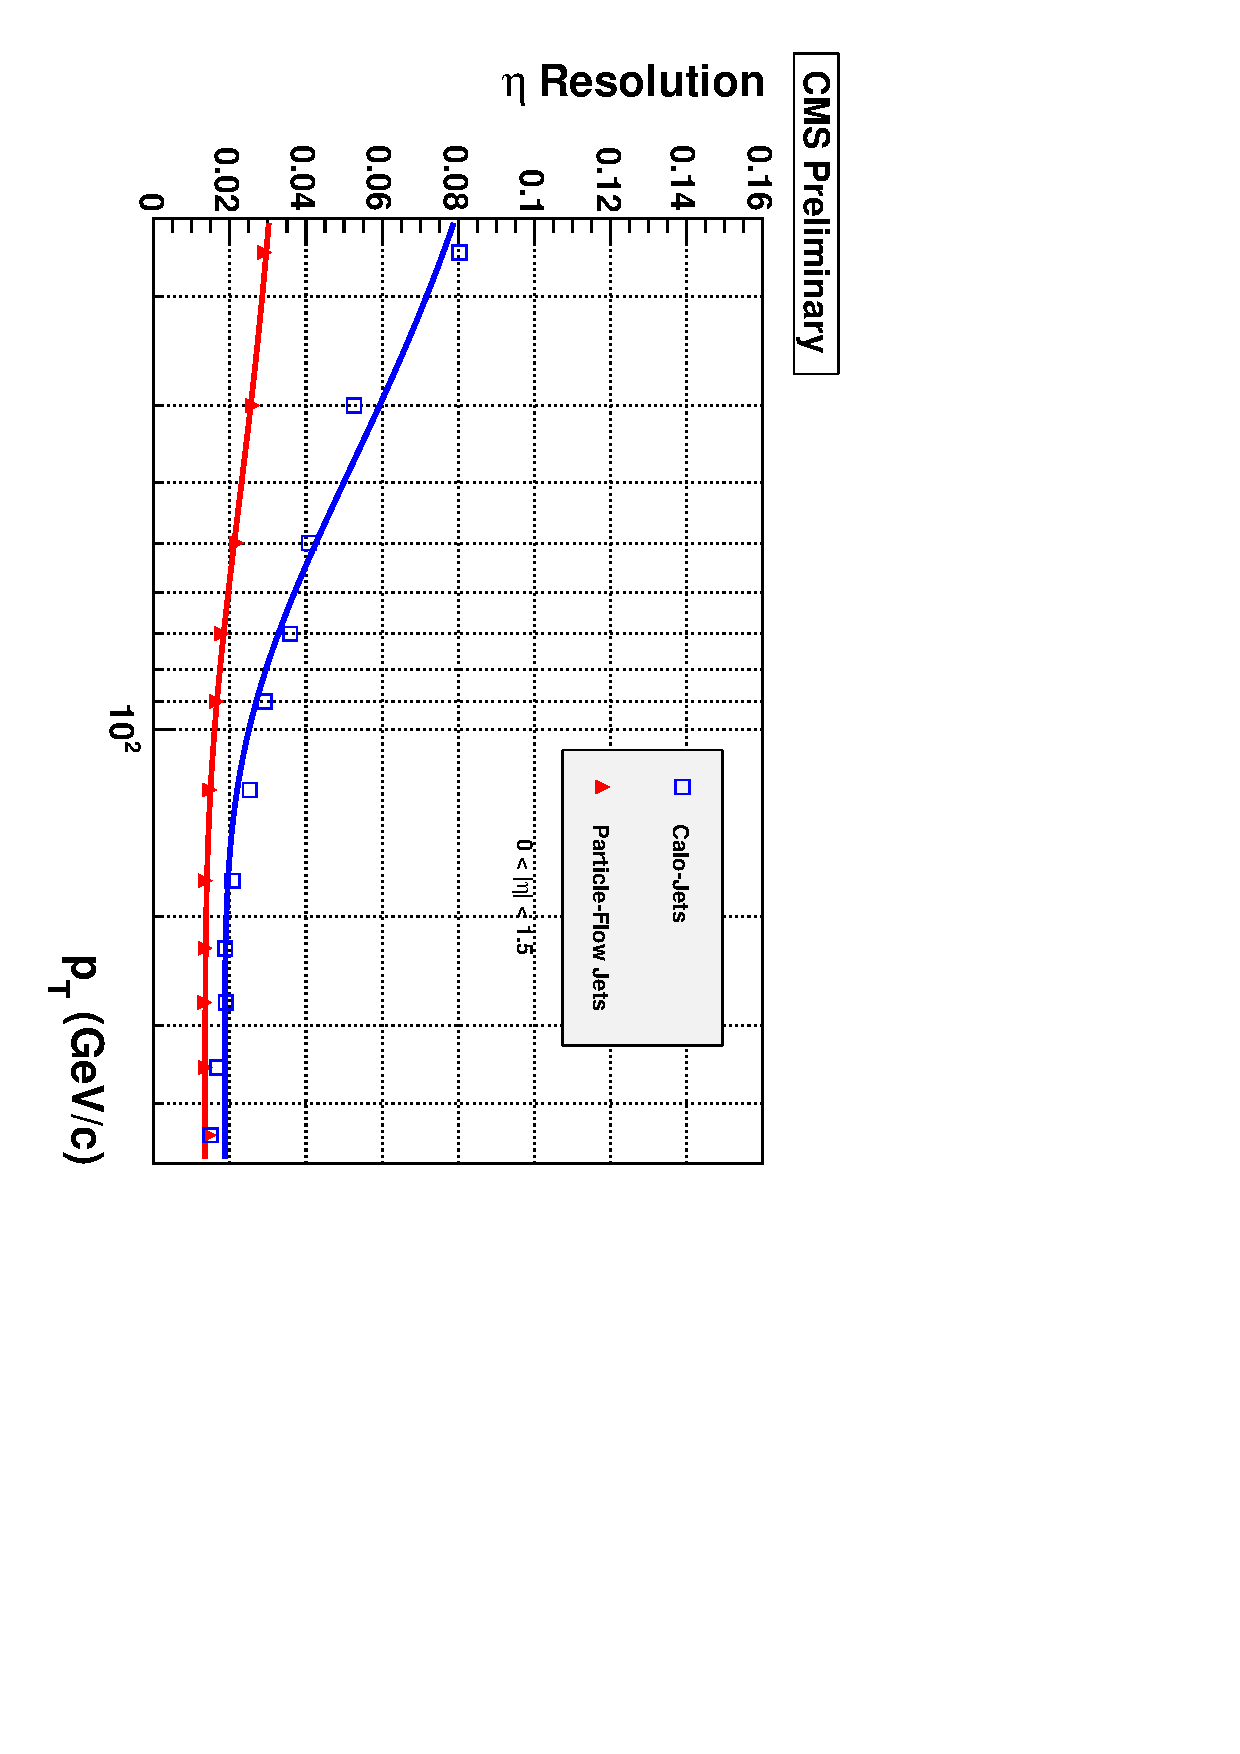
\includegraphics[width=0.45\textwidth]{fig/pf_jet_etares}}\quad
\subfloat[$\phi$]{\label{fig:reco_pf_jet_phires}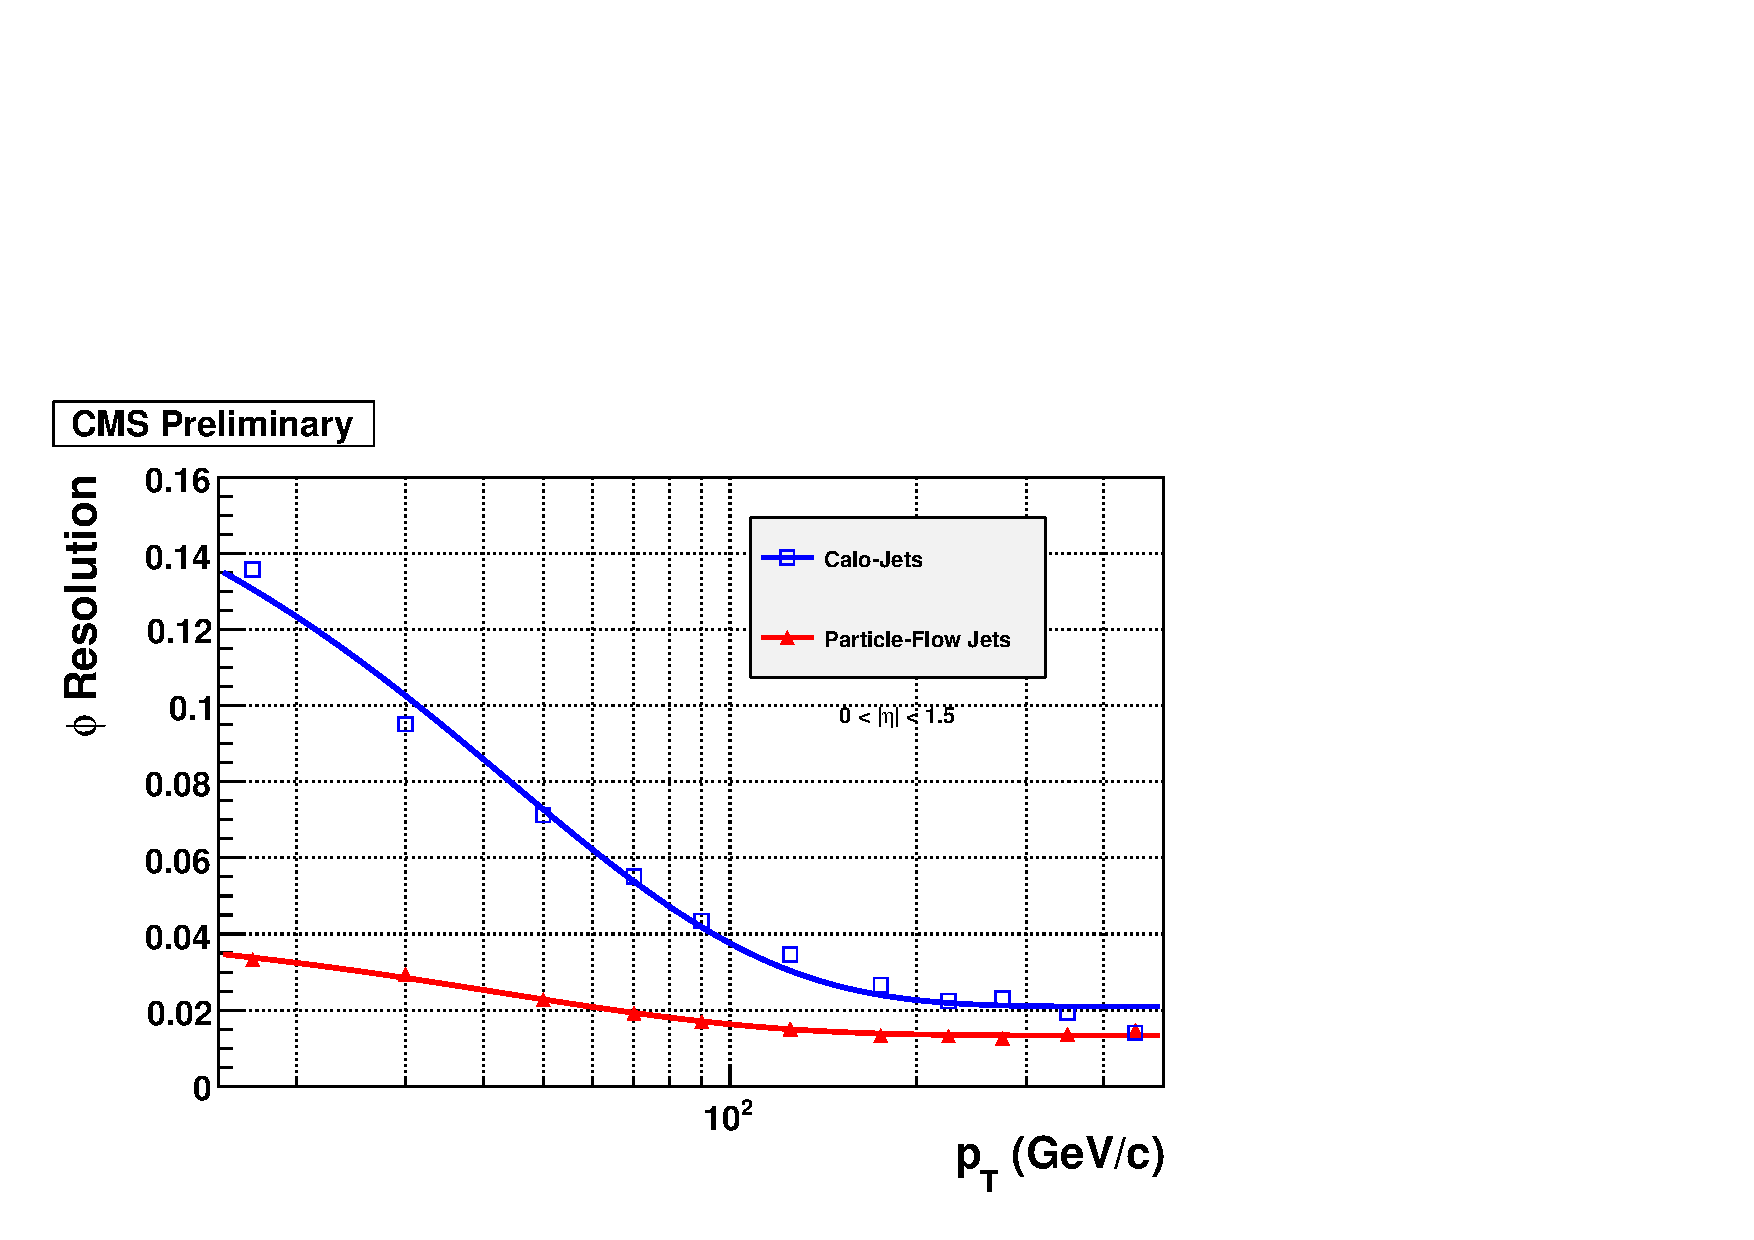
\includegraphics[width=0.45\textwidth]{fig/pf_jet_phires}}\quad
\caption[Jet angular resolution (\acs{RMS}) as a function of \Pt]{Jet angular
  resolution (\ac{RMS}) as a function of \Pt for \subref{fig:reco_pf_jet_etares}
  $\eta$ and \subref{fig:reco_pf_jet_phires} $\phi$. Calo-jets are shown as open
  squares and \ac{PF} jets as upward triangles. The curves are fit with an
  exponential function of $\Pt$~\cite{cms_pf_pas}.}
\label{fig:reco_pf_jet_angularres}
\end{figure}

\begin{figure}[htbp!]
\centering
\subfloat[$\sigma(\MET)/\MET^{\textrm{true}}$]{\label{fig:reco_pf_met_metres}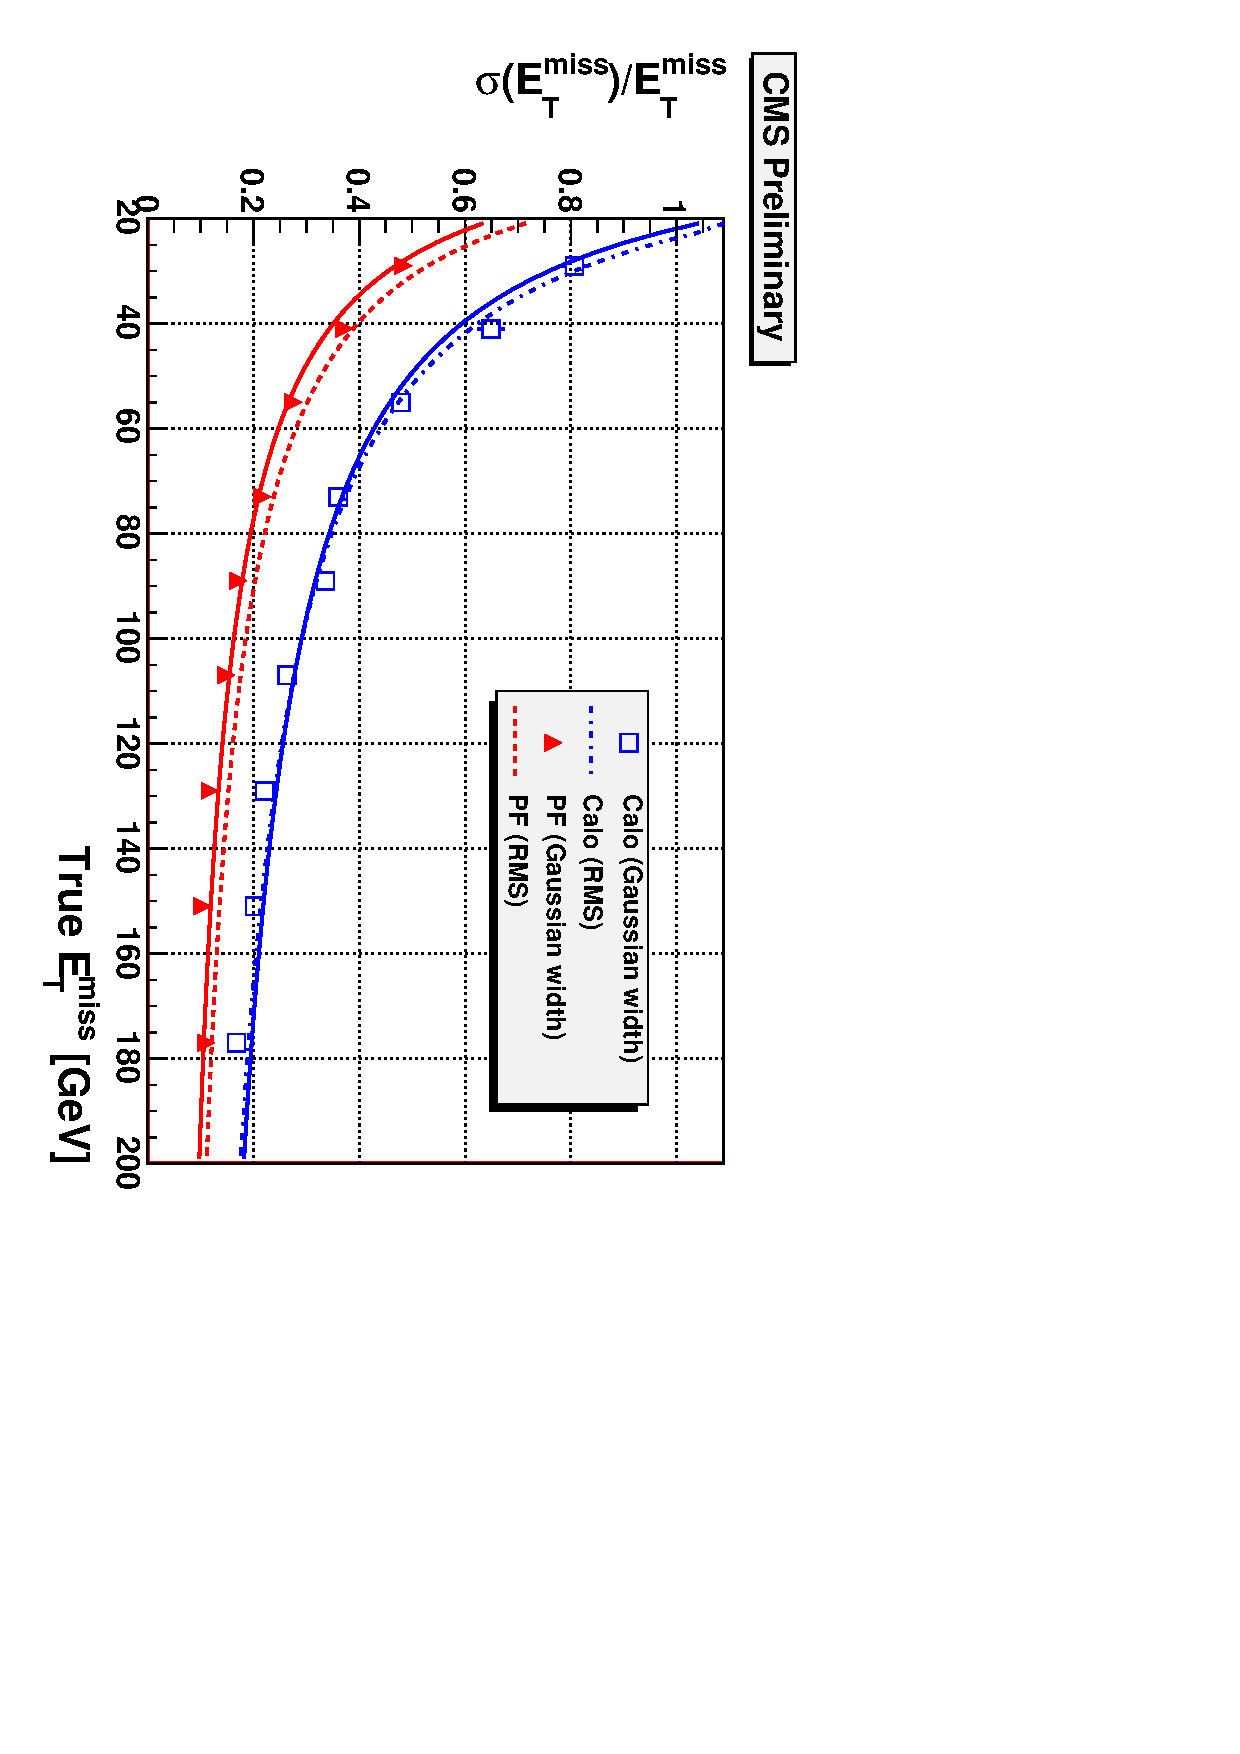
\includegraphics[width=0.45\textwidth]{fig/pf_met_metres}}\quad
\subfloat[$\sigma(\phi)$]{\label{fig:reco_pf_met_phires}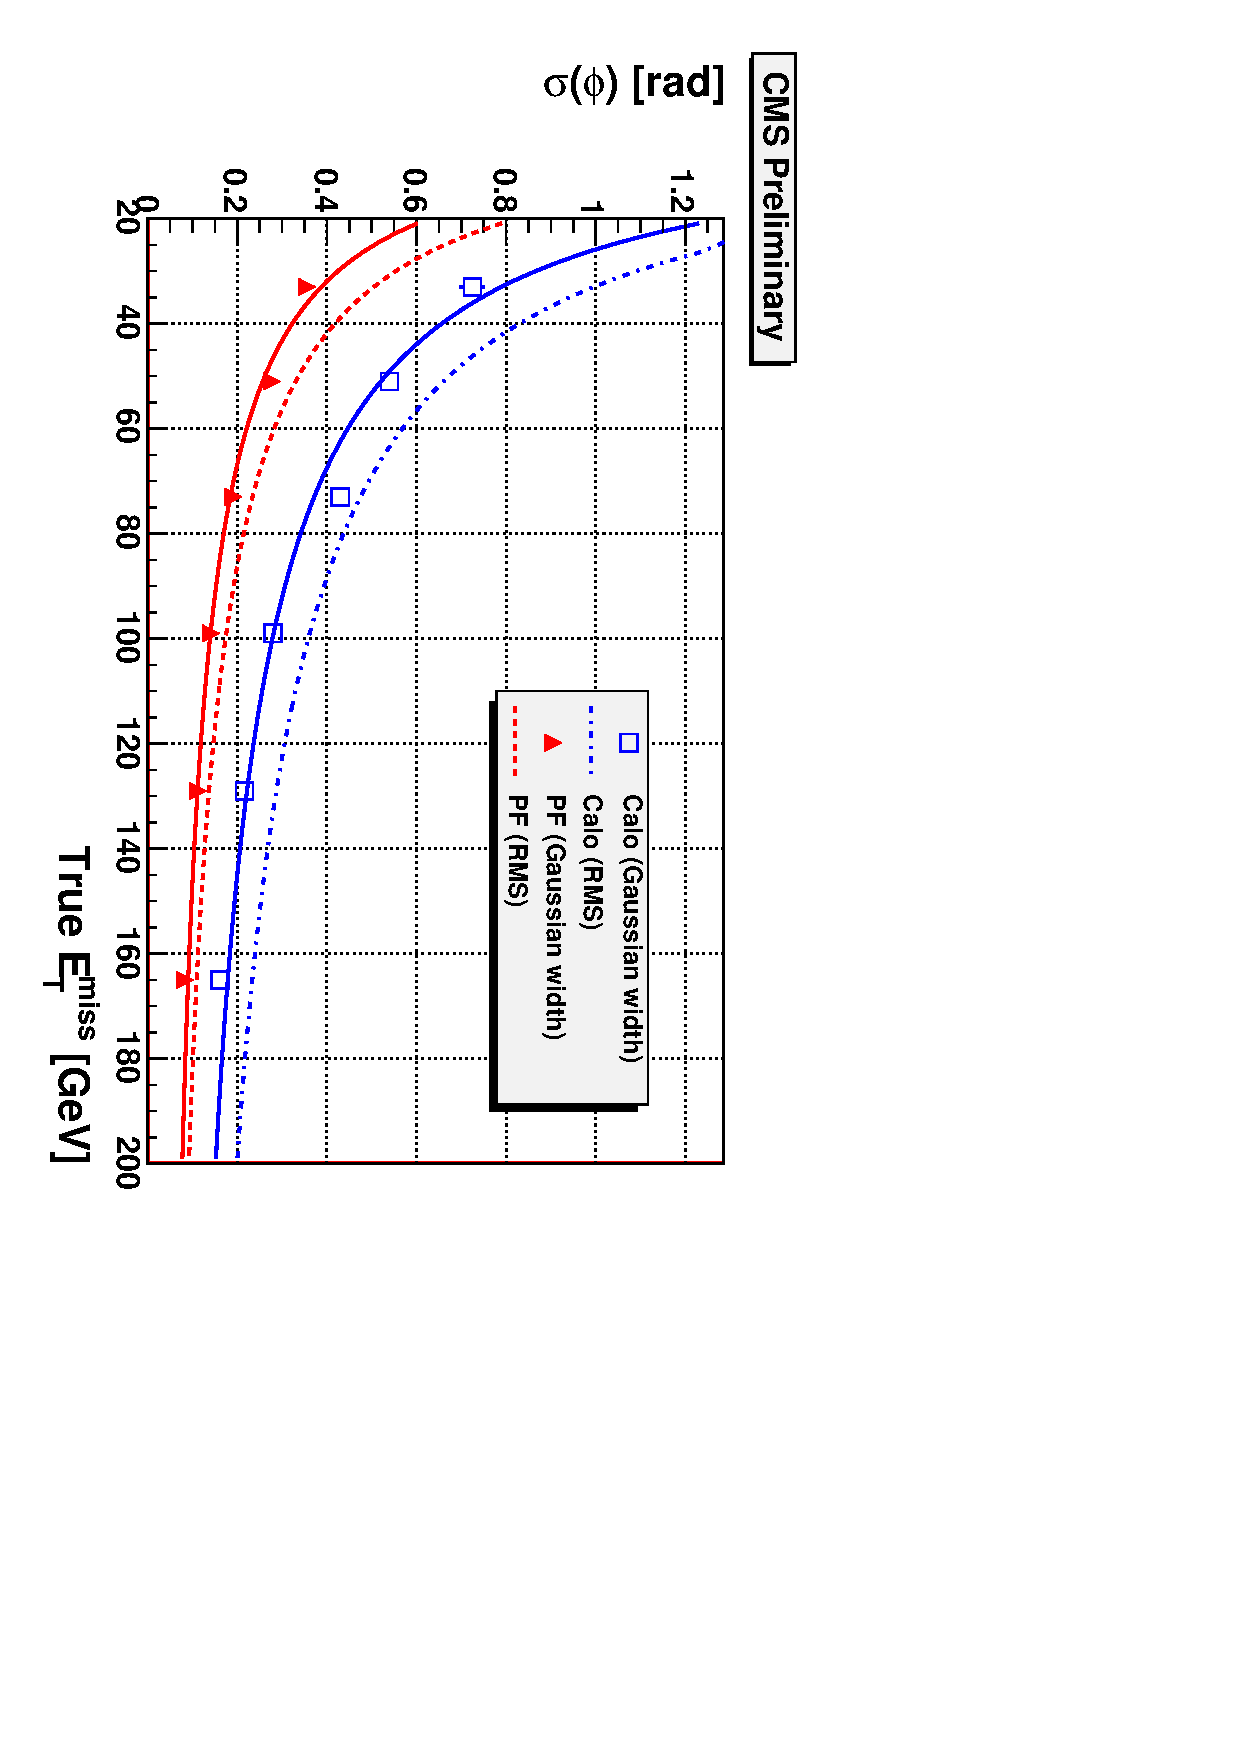
\includegraphics[width=0.45\textwidth]{fig/pf_met_phires}}\quad
\caption[\acl{PF} \MET energy and angular resolution in \ttbar events]{\subref{fig:reco_pf_met_metres} $\sigma(\MET)/\MET^{\textrm{true}}$
  and \subref{fig:reco_pf_met_phires} $\sigma(\phi)$ as a function of true \MET
  in \ttbar events as determined by a Gaussian fit to each
  $\MET^{\textrm{true}}$ bin. Squares represent Calo-\MET, and upwards triangles
  \ac{PF} \MET. The solid curves ares fits through these points. The dashed
  lines indicate the \ac{RMS} width of each bin~\cite{cms_pf_pas}.}
 \label{fig:reco_pf_met_res}
\end{figure}
